% Source of the figure decomposition-example.pdf: the square decomposition of the counterexample graph (a), here with
% c(u,v) = 2. The edges ua, us, sb, ta, tv, vb form F and are drawn from tail to head; the pieces are the squares
% S_1 = {u}, S_2 = {a,b}, S_3 = {v} and the links {s}, {t}. Compile with pdfLaTeX; the PDF is included in the
% manuscript at its natural size.
\documentclass[tikz,border=1pt]{standalone}
\usepackage[T1]{fontenc}
\pdfinfoomitdate=1 \pdftrailerid{} \pdfsuppressptexinfo=-1
\usetikzlibrary{arrows.meta,shapes.geometric}
\definecolor{fblue}{RGB}{31,102,178}
\tikzset{
  vertex/.style={circle, fill=black, inner sep=0pt, minimum size=2.2mm},
  terminal/.style={circle, fill=black, inner sep=0pt, minimum size=3mm},
  edge/.style={line width=0.7pt},
  square/.style={rounded corners=4pt, fill=gray!14, draw=gray!75!black, line width=0.9pt},
  link/.style={ellipse, fill=gray!32, draw=gray!75!black, line width=0.6pt, inner sep=0pt,
               minimum width=11mm, minimum height=8mm},
  fedge/.style={line width=0.9pt, fblue, dash pattern=on 3pt off 1.6pt, -{Stealth[length=2.4mm, width=2mm]}}}
\begin{document}
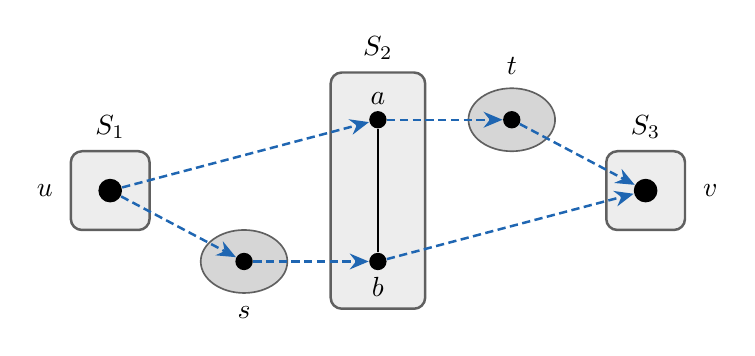
\begin{tikzpicture}[x=1cm, y=1cm]
  % pieces
  \draw[square] (-0.5,-0.5) rectangle (0.5,0.5);
  \draw[square] (2.8,-1.5) rectangle (4.0,1.5);
  \draw[square] (6.3,-0.5) rectangle (7.3,0.5);
  \node[above=1pt] at (0,0.5)   {$S_1$};
  \node[above=1pt] at (3.4,1.5) {$S_2$};
  \node[above=1pt] at (6.8,0.5) {$S_3$};
  \node[link] (ls) at (1.7,-0.9) {};
  \node[link] (lt) at (5.1,0.9)  {};
  % vertices
  \node[terminal] (u) at (0,0) {};
  \node[terminal] (v) at (6.8,0) {};
  \node[vertex] (a) at (3.4,0.9)  {};
  \node[vertex] (b) at (3.4,-0.9) {};
  \node[vertex] (s) at (1.7,-0.9) {};
  \node[vertex] (t) at (5.1,0.9)  {};
  \node[left=3pt]  at (-0.5,0) {$u$};
  \node[right=3pt] at (7.3,0)  {$v$};
  \node[above=2pt] at (a) {$a$};
  \node[below=2pt] at (b) {$b$};
  \node[below=1pt] at (ls.south) {$s$};
  \node[above=1pt] at (lt.north) {$t$};
  % the edge that is not in F
  \draw[edge] (a) -- (b);
  % edges of F, from tail to head
  \draw[fedge] (u) -- (a);
  \draw[fedge] (u) -- (s);
  \draw[fedge] (s) -- (b);
  \draw[fedge] (a) -- (t);
  \draw[fedge] (t) -- (v);
  \draw[fedge] (b) -- (v);
\end{tikzpicture}
\end{document}
